\tR{It can be used to quantify the uncertainity associated with a given
estimator or statistical learning method.}\\

\begin{figure}[H]
	\begin{center}
		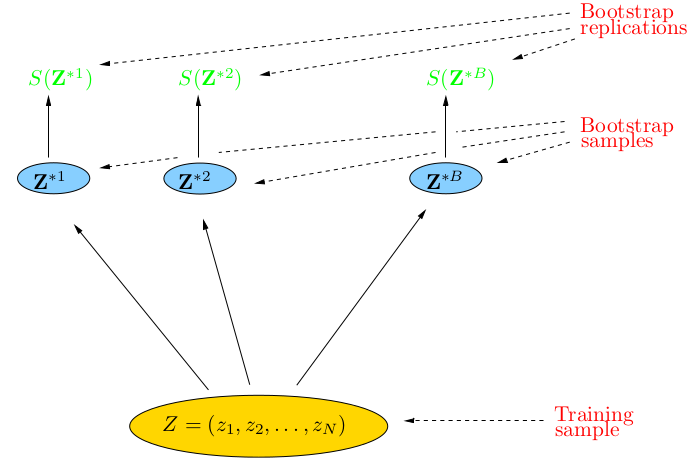
\includegraphics[width=.7\textwidth]{./chap/1chap/4sec/3_bootstrap.png}
	\end{center}
	\caption{Schematic of the bootstrap process}
	\label{fig:3_bootstrap}
\end{figure}

The basic idea is to randomly draw datasets with replacement from the training data, each sample
the same size as the original training set. This is done $B$ times, producing $B$ bootstrap datasets.
$S(\bm{Z})$ is any quantity computed from the data $\bm{Z}$. From the bootstrap sampling we can
estimate any aspect of the distribution of $S(\bm{Z})$, for example its variance:
\begin{center}
\enc{
$\hat{\V{S(\bm{Z})}}=\dfrac{1}{B-1}\su{{b=1}}{B}\left(S(\bm{Z}^{*b})-\overline{S}^{*}\right)^{2}$}
\end{center}
with $\overline{S}^{*}=\dfrac{1}{B}\su{{b=1}}{B}S(\bm{Z}^{*b})$
%\tB{We wish to minimize $\V{\alpha X+(1-\alpha)Y}$ (the risk)} one can
%show that the value that minimze the risk is : 
%\begin{center}
%\encV{$
%\alpha = \dfrac{\sigma_{Y}^{2}-\sigma_{XY}}{\sigma_{X}^{2}\sigma_{Y}^{2}-2\sigma_{XY}}
%$}
%\end{center}
%and $\sigma_{XY}=Cov(X,Y)$\\
%In reality, the quantities $\sigma_{X}^{2},\sigma_{Y}^{2}$ and $\sigma_{XY}$ are unknown.\\
%
%\tB{We can compute the standard error of these bootstrap estimates}
%using the formula:
%\begin{center}
%\encV{$
%SE_{B}\left( \hat{\alpha} \right)=
%\sqrt{\dfrac{1}{B-1}\su{{r=1}}{B}\left( \hat{\alpha}^{*r}-\dfrac{1}{B}\su{{r'=1}}{B}\hat{\alpha}^{*r'} \right)^{2}}
%$}
%\end{center}
